% =====================================================================
%  เล่มรายงานโครงงานคอมพิวเตอร์ (template v2)
%  สาขาวิชาวิทยาการคอมพิวเตอร์ วิทยาลัยการคอมพิวเตอร์ มหาวิทยาลัยขอนแก่น
%
%  Compile: XeLaTeX + Biber
%    Overleaf : Menu > Settings > Compiler = XeLaTeX (biber ทำงานอัตโนมัติ)
%    เครื่องตนเอง: latexmk   (อ่านค่าจาก .latexmkrc)
%
%  นักศึกษาแก้ไขเฉพาะ: ไฟล์นี้ (ข้อมูลโครงงาน), frontmatter/, chapters/,
%  backmatter/, references.bib และ images/
%  ไม่ต้องแก้ไฟล์ .cls / .sty — รูปแบบทั้งหมดเป็นไปตาม
%  "คู่มือการจัดทำเอกสารโครงงานคอมพิวเตอร์" ของสาขาวิชาแล้ว
% =====================================================================
\documentclass[final]{cskkuproject}
% ชนิดเล่ม (เลือก 1 อย่าง):
%   progress1  รายงานความก้าวหน้าโครงงาน ครั้งที่ 1
%   progress2  รายงานความก้าวหน้าโครงงาน ครั้งที่ 2
%   final      เอกสารโครงงานฉบับสมบูรณ์
% ตัวเลือกเพิ่มเติม เช่น \documentclass[final,plainnumbering]{cskkuproject}
%   plainnumbering     เลขหัวข้อแบบ 1. / 1.1 / 1.1.1 / (1)
%   boldheadings       หัวข้อย่อยตัวหนา
%   chapterfloats      เลขภาพ/ตารางแยกตามบท (2.1, 2.2, ...)
%   chapterpagenumber  แสดงเลขหน้าในหน้าแรกของบท
%   titleasis          ไม่แปลงชื่อภาษาอังกฤษบนปกเป็นตัวพิมพ์ใหญ่
%   englishbook        เล่มภาษาอังกฤษทั้งเล่ม
%   mermaid            ใช้แผนภาพ Mermaid (ดู README.md)

% ---------------------------------------------------------------------
% 1) ข้อมูลโครงงาน (ใช้สร้างปก บทคัดย่อ และกิตติกรรมประกาศอัตโนมัติ)
% ---------------------------------------------------------------------
\projectCode{CS 2568/xx}             % CS/IT พ.ศ./กลุ่ม ตามที่สาขากำหนด
\titleTH{ชื่อโครงงานภาษาไทย}
\titleEN{Project Title in English}
% ชื่อยาวเกิน 2 บรรทัด ระบบจัดเป็นสามเหลี่ยมกลับหัวให้เอง
% ตัดบรรทัดเองได้ด้วย \\ เช่น \titleTH{ระบบ...\\ สำหรับ...}

% นักศึกษา (สูงสุด 3 คน) — คำนำหน้าชื่อเขียนติดกับชื่อ ไม่เว้นวรรค
\firstStudentID{6xxxxxxxx-x}
\firstStudentPrefixTH{นาย}
\firstStudentNameTH{ชื่อ นามสกุล}
\firstStudentPrefixEN{Mr.}
\firstStudentNameEN{Firstname Lastname}

% คนที่ 2 และ 3: เว้นว่างไว้ถ้าไม่มี
\secondStudentID{}
\secondStudentPrefixTH{}
\secondStudentNameTH{}
\secondStudentPrefixEN{}
\secondStudentNameEN{}

\thirdStudentID{}
\thirdStudentPrefixTH{}
\thirdStudentNameTH{}
\thirdStudentPrefixEN{}
\thirdStudentNameEN{}

% อาจารย์ที่ปรึกษา — ตำแหน่งทางวิชาการเขียนติดกับชื่อ เช่น ผศ.ดร.ชื่อ นามสกุล
\advisorTH{ผศ.ดร.ชื่อ นามสกุล}
\advisorEN{Asst. Prof. Firstname Lastname, Ph.D.}
% \coadvisorTH{อ.ดร.ชื่อ นามสกุล}          % อาจารย์ที่ปรึกษาร่วม (ถ้ามี)
% \coadvisorEN{Firstname Lastname, Ph.D.}

% รายวิชาและภาคการศึกษา (ตรวจสอบรหัสวิชาตามหลักสูตรของรุ่น)
\courseCode{CP354 772}
\courseName{โครงงานคอมพิวเตอร์ 2}
\semester{2}
\academicYearTH{2568}
\submitMonthTH{มีนาคม}                % เดือนและปีที่ส่งเล่ม (บรรทัดสุดท้ายของปก)
\submitYearTH{2569}

% หลักสูตร (ค่าเริ่มต้นคือ วท.บ. วิทยาการคอมพิวเตอร์ — แก้เมื่อไม่ตรง)
% \degreeTH{วิทยาศาสตรบัณฑิต}   \degreeEN{Bachelor of Science}
% \majorTH{วิทยาการคอมพิวเตอร์}  \majorEN{Computer Science}

% คำสำคัญ (แสดงท้ายบทคัดย่อ) 3–5 คำ
\keywordsTH{คำสำคัญ 1, คำสำคัญ 2, คำสำคัญ 3}
\keywordsEN{Keyword 1, Keyword 2, Keyword 3}

% ไฟล์รายการอ้างอิง
\addbibresource{references.bib}

% สารบัญแสดงบท หัวข้อใหญ่ (4.1) และหัวข้อย่อยระดับ 1 (4.1.1) ตามคู่มือข้อ 13
% ถ้าต้องการแสดงเฉพาะหัวข้อใหญ่ ให้เอา % หน้าบรรทัดถัดไปออก
% \setcounter{tocdepth}{1}

\begin{document}

% ---------------------------------------------------------------------
% 2) ปกนอก ปกใน และส่วนต้น (เลขหน้า ก ข ค ...)
% ---------------------------------------------------------------------
\makecover            % ปกนอก
\makeinnercover       % ปกใน (ข้อความเหมือนปกนอก)
\frontmatter

\begin{abstractTH}
% =====================================================================
% บทคัดย่อภาษาไทย (คู่มือข้อ 11)
% ส่วนหัว (ชื่อผู้เขียน ปี ชื่อเรื่อง ปริญญา สาขา อาจารย์ที่ปรึกษา) และคำสำคัญ
% ระบบสร้างให้อัตโนมัติจากข้อมูลใน main.tex — เขียนเฉพาะเนื้อหาบทคัดย่อ
%
% หลักการเขียน: ไม่เกิน 1 หน้า (ประมาณ 300 คำ) เป็นความเรียงย่อหน้าเดียวหรือสองย่อหน้า
%   วัตถุประสงค์ -> วิธีการ/เครื่องมือ -> ผลการดำเนินงาน (มีตัวเลข) -> ประโยชน์
%   ไม่อ้างอิงเอกสาร ไม่ใส่ภาพ ตาราง หรือสมการ
% *** ลบข้อความตัวอย่างแล้วเขียนบทคัดย่อของตนเอง ***
% =====================================================================
โครงงานนี้มีวัตถุประสงค์เพื่อพัฒนาระบบ\ldots{} สำหรับ\ldots{} เพื่อแก้ปัญหา\ldots{}
ระบบพัฒนาเป็นเว็บแอปพลิเคชันด้วย\ldots{} และใช้ฐานข้อมูล\ldots{}
ประกอบด้วยฟังก์ชันหลัก ได้แก่ \ldots{} \ldots{} และ \ldots{}
ผลการทดสอบการยอมรับของผู้ใช้จำนวน\ldots{} คน พบว่าระบบทำงานได้ถูกต้องตามกรณีทดสอบร้อยละ\ldots{}
และผู้ใช้มีความพึงพอใจในระดับ\ldots{} (ค่าเฉลี่ย\ldots{} จาก 5)
ระบบที่พัฒนาขึ้นช่วยลดเวลาในการ\ldots{} จากเดิม\ldots{} เหลือ\ldots{}

\end{abstractTH}

\begin{abstractEN}
% =====================================================================
% ABSTRACT (คู่มือข้อ 11)
% The header (authors, year, title, degree, advisor) and keywords are
% generated from main.tex. Write only the abstract text here.
%
% Content must match the Thai abstract. Use the past tense for the
% objectives and methods, and the present tense for results and conclusions.
% *** Delete the sample text and write your own abstract ***
% =====================================================================
This project aimed to develop a\ldots{} system for\ldots{} in order to solve\ldots{}
The system was developed as a web application using\ldots{} with\ldots{} as the database.
Its main functions are\ldots, \ldots, and\ldots{}
User acceptance testing with\ldots{} users shows that the system passes\ldots{} percent
of the test cases, and user satisfaction is at the\ldots{} level (mean\ldots{} out of 5).
The system reduces the time required for\ldots{} from\ldots{} to\ldots{}

\end{abstractEN}

\begin{acknowledgement}
% =====================================================================
% กิตติกรรมประกาศ (คู่มือข้อ 12) — ไม่เกิน 1 หน้า
% ระบบใส่ "ผู้จัดทำ" และรายชื่อนักศึกษาท้ายหน้าให้อัตโนมัติ
% *** แก้ข้อความตัวอย่างให้เป็นของตนเอง ***
% =====================================================================
โครงงานนี้สำเร็จลุล่วงได้ด้วยความกรุณาจาก\ldots{} อาจารย์ที่ปรึกษาโครงงาน
ที่ได้ให้คำแนะนำ คำปรึกษา และตรวจแก้ไขรายงานตลอดระยะเวลาการดำเนินงาน
ผู้จัดทำขอขอบพระคุณเป็นอย่างสูง

ขอขอบพระคุณคณาจารย์สาขาวิชาวิทยาการคอมพิวเตอร์ วิทยาลัยการคอมพิวเตอร์ มหาวิทยาลัยขอนแก่น
ที่ได้ถ่ายทอดความรู้อันเป็นพื้นฐานสำคัญในการทำโครงงาน
และขอขอบคุณ\ldots{} ที่ให้ข้อมูลและสละเวลาร่วมทดสอบระบบ

ท้ายนี้ ขอขอบพระคุณบิดา มารดา และครอบครัว ที่ให้การสนับสนุนและเป็นกำลังใจตลอดมา

\end{acknowledgement}

\makecontents         % สารบัญ -> สารบัญตาราง -> สารบัญภาพ -> สารบัญสมการ (ข้ามรายการที่ไม่มี)

\begin{symbols}       % รายการสัญลักษณ์และคำย่อ (ลบทั้ง 3 บรรทัดถ้าไม่มี)
% =====================================================================
% รายการสัญลักษณ์และคำย่อ (คู่มือข้อ 16) — ใส่เฉพาะเมื่อมีการใช้ในเล่ม
% \symbolitem{สัญลักษณ์หรือคำย่อ}{ความหมาย}  เรียงตามตัวอักษร
% ถ้าไม่มี ให้ลบบล็อก \begin{symbols} ... \end{symbols} ใน main.tex
% =====================================================================
\symbolitem{API}{Application Programming Interface}
\symbolitem{ER}{Entity-Relationship}
\symbolitem{FR}{Functional Requirement (ความต้องการเชิงฟังก์ชัน)}
\symbolitem{NFR}{Non-functional Requirement (ความต้องการที่ไม่ใช่เชิงฟังก์ชัน)}
\symbolitem{UAT}{User Acceptance Testing (การทดสอบการยอมรับของผู้ใช้)}
\symbolitem{UML}{Unified Modeling Language}
\symbolitem{$\bar{x}$}{ค่าเฉลี่ย}
\symbolitem{S.D.}{ส่วนเบี่ยงเบนมาตรฐาน}

\end{symbols}

% ---------------------------------------------------------------------
% 3) เนื้อเรื่อง 5 บท (เลขหน้า 1 2 3 ...) — ชื่อบทกำหนดตามคู่มือแล้ว
% ---------------------------------------------------------------------
\mainmatter

\chapter{\chapteronetitle}      % บทนำ
% =====================================================================
% บทที่ 1 บทนำ (คู่มือข้อ 17.1)
%   1.1 ความเป็นมาและความสำคัญของปัญหา
%   1.2 วัตถุประสงค์
%   1.3 เป้าหมายและขอบเขต
%   1.4 ประโยชน์ที่คาดว่าจะได้รับ
% *** ก่อนส่ง: ลบข้อความตัวอย่าง (...) และคำแนะนำที่ขึ้นต้นด้วย % ได้ตามต้องการ ***
% =====================================================================

\section{ความเป็นมาและความสำคัญของปัญหา}
\label{sec:background}

% เริ่มจากสภาพปัญหาในภาพกว้าง แล้วเจาะจงลงมาที่ปัญหาที่โครงงานนี้แก้
% ระบุผลกระทบของปัญหาเป็นตัวเลขเมื่อทำได้ และอ้างอิงแหล่งที่มาด้วย \cite{key}

ปัจจุบัน\ldots{} มีบทบาทสำคัญต่อ\ldots{} จากการสำรวจของ\ldots{}~\cite{thesismgmt2023}
พบว่า\ldots{} อย่างไรก็ตาม การดำเนินงานในปัจจุบันยังมีปัญหา\ldots{}
ทำให้ผู้ใช้ต้องใช้เวลา\ldots{} และเกิดความผิดพลาดในการ\ldots{}

ผู้จัดทำจึงพัฒนาระบบ\ldots{} เพื่อ\ldots{} โดยนำแนวคิด\ldots{}
มาประยุกต์ใช้ร่วมกับเทคโนโลยี\ldots{}

\section{วัตถุประสงค์}
\label{sec:objectives}

% เขียนเป็นข้อ ขึ้นต้นด้วย "เพื่อ" และวัดผลได้ (จะสรุปผลเทียบกับข้อเหล่านี้ในบทที่ 5)

\begin{enumerate}
  \item เพื่อศึกษาและวิเคราะห์กระบวนการ\ldots{}
  \item เพื่อออกแบบและพัฒนาระบบ\ldots{}
  \item เพื่อทดสอบและประเมินความพึงพอใจของผู้ใช้ที่มีต่อระบบ\ldots{}
\end{enumerate}

\section{เป้าหมายและขอบเขต}
\label{sec:scope}

\subsection{เป้าหมาย}

% ระบุสิ่งที่จะได้เมื่อจบโครงงานในเชิงปริมาณหรือคุณภาพ เช่น ใครใช้ ใช้ทำอะไร ใช้ได้กี่คน

ได้ระบบ\ldots{} ที่ผู้ใช้\ldots{} สามารถใช้\ldots{} ได้ผ่านเว็บเบราว์เซอร์
รองรับผู้ใช้\ldots{} บทบาท ได้แก่ \ldots{}

\subsection{ขอบเขตของระบบ}

% ระบบงาน: ระบุความต้องการเชิงฟังก์ชันและที่ไม่ใช่เชิงฟังก์ชันโดยสรุป (รายละเอียดอยู่ในบทที่ 4)
% งานวิจัย: ระบุกระบวนการทดลอง ข้อมูลที่ใช้ สภาพแวดล้อมการทดลอง และวิธีวัดผล

\begin{enumerate}
  \item ผู้ใช้ทั่วไปสามารถ\ldots{}
  \begin{enumerate}
    \item สมัครสมาชิกและเข้าสู่ระบบ
    \item \ldots{}
  \end{enumerate}
  \item ผู้ดูแลระบบสามารถ\ldots{}
  \item ระบบทำงานบนเว็บเบราว์เซอร์ Google Chrome และ Microsoft Edge รุ่นล่าสุด
  \item ระบบติดตั้งบนเครื่องแม่ข่ายของ\ldots{} ทดสอบกับข้อมูลจำนวน\ldots{} รายการ
\end{enumerate}

% ข้อจำกัดของระบบให้เขียนในบทที่ 5 หัวข้อ 5.2 (คู่มือข้อ 17.5)

\section{ประโยชน์ที่คาดว่าจะได้รับ}
\label{sec:benefits}

\begin{enumerate}
  \item ผู้ใช้ลดเวลาในการ\ldots{}
  \item หน่วยงานมีข้อมูล\ldots{} ที่ถูกต้องและเป็นปัจจุบันสำหรับ\ldots{}
  \item ผู้จัดทำได้ความรู้และทักษะด้าน\ldots{}
\end{enumerate}


\chapter{\chaptertwotitle}      % งานวิจัยและทฤษฎีที่เกี่ยวข้อง
% =====================================================================
% บทที่ 2 งานวิจัยและทฤษฎีที่เกี่ยวข้อง (คู่มือข้อ 17.2)
%   2.1 งานวิจัย โครงงาน ระบบงาน หรือโปรแกรมที่เกี่ยวข้อง
%       (ส่วนที่คล้ายกัน และส่วนที่แตกต่างจากโครงงานนี้)
%   2.2 หลักการและทฤษฎีที่นำมาใช้ในโครงงาน
%
% การอ้างอิง: \cite{key} -> [1]   \cite{a,b} -> [1, 2]   \cite{a,b,c} -> [1-3]
% เลขอ้างอิงเรียงตามลำดับที่อ้างครั้งแรกในเล่ม และแสดงในหน้า "เอกสารอ้างอิง" ให้อัตโนมัติ
% *** ก่อนส่ง: ลบข้อความตัวอย่าง (...) ***
% =====================================================================

\section{งานวิจัย โครงงาน และระบบงานที่เกี่ยวข้อง}
\label{sec:related}

% สำหรับแต่ละงาน: ใครทำ ทำอะไร ใช้วิธีใด ได้ผลอย่างไร จุดเด่น/ข้อจำกัด
% และเกี่ยวข้องกับโครงงานนี้อย่างไร (นำแนวคิดใดมาใช้ หรือโครงงานนี้แก้ข้อจำกัดใด)

ผู้จัดทำได้ศึกษางานวิจัยและระบบที่มีลักษณะคล้ายกับโครงงานนี้ จำนวน 4 งาน
ได้แก่ ระบบจัดการวิทยานิพนธ์ออนไลน์~\cite{thesismgmt2023}
ระบบจัดการโครงงานสำหรับรายวิชาวิศวกรรมซอฟต์แวร์~\cite{projmgmt2023}
และโปรแกรมแก้ไขเอกสาร \LaTeX{} ออนไลน์~\cite{overleaf2024,swiftlatex2019}
มีรายละเอียดดังนี้

\subsection{ระบบจัดการวิทยานิพนธ์ออนไลน์}

สมหญิง รักเรียน และสมศักดิ์ ขยันทำ~\cite{thesismgmt2023} พัฒนาระบบ\ldots{}
โดยใช้\ldots{} ผลการทดสอบพบว่า\ldots{}
จุดเด่นของระบบคือ\ldots{} แต่ยังมีข้อจำกัดด้าน\ldots{}
โครงงานนี้นำแนวคิด\ldots{} มาใช้ และเพิ่มความสามารถ\ldots{}

\subsection{ระบบจัดการโครงงานสำหรับรายวิชาวิศวกรรมซอฟต์แวร์}

Somchai และ Wichian~\cite{projmgmt2023} นำเสนอ\ldots{}
ซึ่งคล้ายกับโครงงานนี้ในส่วน\ldots{} แต่แตกต่างกันที่\ldots{}

\subsection{สรุปการเปรียบเทียบ}

การเปรียบเทียบความสามารถของงานที่เกี่ยวข้องกับโครงงานนี้แสดงดังตารางที่~\ref{tab:compare}

\begin{table}[H]
\caption{การเปรียบเทียบความสามารถของงานที่เกี่ยวข้องกับโครงงานนี้}
\label{tab:compare}
\centering
\begin{tabular}{|L{4.6cm}|C{1.9cm}|C{1.9cm}|C{1.9cm}|C{1.9cm}|}
\hline
\textbf{งาน} & \textbf{ความสามารถ A} & \textbf{ความสามารถ B}
  & \textbf{ความสามารถ C} & \textbf{ความสามารถ D} \\ \hline
ระบบจัดการวิทยานิพนธ์~\cite{thesismgmt2023} & \cmark & \cmark & -- & -- \\ \hline
ระบบจัดการโครงงาน~\cite{projmgmt2023}      & \cmark & --     & \cmark & -- \\ \hline
Overleaf~\cite{overleaf2024}                 & --     & \cmark & \cmark & -- \\ \hline
\textbf{โครงงานนี้}                          & \cmark & \cmark & \cmark & \cmark \\ \hline
\end{tabular}
\end{table}

จากตารางที่~\ref{tab:compare} ยังไม่มีงานใดที่มีความสามารถ D
โครงงานนี้จึงพัฒนาระบบที่มีความสามารถครบทั้ง 4 ด้าน

\section{หลักการและทฤษฎีที่เกี่ยวข้อง}
\label{sec:theory}

% อธิบายเฉพาะหลักการ ทฤษฎี และเทคโนโลยีที่ "ใช้จริง" ในโครงงาน พร้อมอ้างอิง
% ไม่ต้องอธิบายความรู้ทั่วไปที่ไม่ได้นำมาใช้

\subsection{สถาปัตยกรรมแบบ REST}

REST (Representational State Transfer) เป็นรูปแบบสถาปัตยกรรมของระบบบนเครือข่าย
ที่นำเสนอโดย Fielding~\cite{fielding2000} มีหลักการสำคัญ ได้แก่
\begin{enumerate}
  \item การแยกส่วนผู้ใช้บริการและผู้ให้บริการ (Client--Server)
  \item การไม่เก็บสถานะของผู้ใช้บริการไว้ที่ผู้ให้บริการ (Stateless)
  \item การใช้ส่วนต่อประสานที่เป็นรูปแบบเดียวกัน (Uniform interface)
\end{enumerate}
โครงงานนี้ใช้หลักการดังกล่าวออกแบบ API ของระบบในหัวข้อ~\ref{sec:design}

\subsection{ระบบจัดเตรียมเอกสาร \LaTeX}

\LaTeX{} เป็นระบบจัดเตรียมเอกสารที่แยกเนื้อหาออกจากรูปแบบ~\cite{latex2023}
\ldots{}

\subsection{คอนเทนเนอร์ด้วย Docker}

Docker เป็นแพลตฟอร์มสำหรับสร้างและรันแอปพลิเคชันในคอนเทนเนอร์~\cite{docker2024}
\ldots{}


\chapter{\chapterthreetitle}    % วิธีการดำเนินงาน
% =====================================================================
% บทที่ 3 วิธีการดำเนินงาน (คู่มือข้อ 17.3)
% อธิบายขั้นตอนและวิธีการดำเนินงาน และเครื่องมือที่ใช้ในการทำโครงงาน
% *** ก่อนส่ง: ลบข้อความตัวอย่าง (...) ***
% =====================================================================

\section{ขั้นตอนการดำเนินงาน}
\label{sec:method}

โครงงานนี้ดำเนินงานตามแนวทาง\ldots{} (เช่น Agile แบบ Scrum หรือ Waterfall)
แบ่งเป็น 5 ขั้นตอน ดังภาพที่~\ref{fig:method}

% แผนภาพขั้นตอนวาดด้วย TikZ (แก้ข้อความในวงเล็บปีกกาได้โดยตรง)
% หรือใช้ภาพจากโปรแกรมอื่น: \includegraphics[width=0.9\linewidth]{images/ชื่อไฟล์}
\begin{figure}[H]
\centering
\begin{tikzpicture}[
    node distance=7bp and 10bp,
    stage/.style={draw=black!70, fill=black!4, rounded corners=3pt, align=center,
      font=\normalfont\small, minimum height=34bp, text width=64bp, inner sep=3bp},
    arr/.style={-{Stealth[length=5bp]}, line width=0.8pt, draw=black!60}]
  \node[stage] (s1) {ศึกษาปัญหาและ\\ความต้องการ};
  \node[stage, right=of s1] (s2) {วิเคราะห์และ\\ออกแบบระบบ};
  \node[stage, right=of s2] (s3) {พัฒนาระบบ};
  \node[stage, right=of s3] (s4) {ทดสอบและ\\ประเมินผล};
  \node[stage, right=of s4] (s5) {ปรับปรุงและ\\สรุปผล};
  \draw[arr] (s1) -- (s2); \draw[arr] (s2) -- (s3);
  \draw[arr] (s3) -- (s4); \draw[arr] (s4) -- (s5);
  \draw[arr] (s4.south) -- ++(0,-12bp) -| node[pos=0.25, below, font=\normalfont\footnotesize]{พบข้อผิดพลาด} (s3.south);
\end{tikzpicture}
\caption{ขั้นตอนการดำเนินงาน}
\label{fig:method}
\end{figure}

\subsection{ศึกษาปัญหาและรวบรวมความต้องการ}

สัมภาษณ์\ldots{} จำนวน\ldots{} คน และศึกษาเอกสาร\ldots{} เพื่อรวบรวมความต้องการของระบบ

\subsection{วิเคราะห์และออกแบบระบบ}

วิเคราะห์ความต้องการด้วยแผนภาพ UML และออกแบบฐานข้อมูล (รายละเอียดในบทที่ 4)

\subsection{พัฒนาระบบ}

พัฒนาระบบด้วยภาษา\ldots{} และเฟรมเวิร์ก\ldots{} โดยแบ่งการพัฒนาเป็นรอบละ\ldots{} สัปดาห์

\subsection{ทดสอบและประเมินผล}

ทดสอบระบบด้วยกรณีทดสอบ (Test case) และประเมินความพึงพอใจของผู้ใช้ด้วยแบบสอบถาม
โดยวิเคราะห์คะแนนด้วยค่าเฉลี่ยตามสมการที่~\eqref{eq:mean}

% สมการ: เลขสมการในวงเล็บชิดขวาให้อัตโนมัติ (1), (2), ... หรือ (3.1) เมื่อใช้ chapterfloats
%   \eqcaption{ชื่อสมการ} -> แสดงในสารบัญสมการ (สร้างหน้าสารบัญสมการให้เมื่อมีอย่างน้อย 1 สมการ)
%   อ้างถึงในเนื้อหาด้วย สมการที่~\eqref{ชื่อ label} -> "สมการที่ (1)"
%   ข้อความภาษาไทยในสมการเขียนใน \text{...}
\begin{equation}
\bar{x} = \frac{1}{n}\sum_{i=1}^{n} x_i
\eqcaption{ค่าเฉลี่ยเลขคณิต}
\label{eq:mean}
\end{equation}
% คำอธิบายสัญลักษณ์ใต้สมการ: คอลัมน์แรกเป็นสัญลักษณ์ (โหมดคณิตศาสตร์) คอลัมน์ที่สองเป็นคำอธิบาย
\begin{eqwhere}
\bar{x} & ค่าเฉลี่ยของคะแนน \\
x_i     & คะแนนของผู้ตอบคนที่ $i$ \\
n       & จำนวนผู้ตอบแบบสอบถาม
\end{eqwhere}

\subsection{ปรับปรุงและสรุปผล}

ปรับปรุงระบบตามผลการทดสอบ และจัดทำรายงานและคู่มือการใช้งาน

\section{เครื่องมือที่ใช้ในการดำเนินงาน}
\label{sec:tools}

\subsection{ฮาร์ดแวร์}

ฮาร์ดแวร์ที่ใช้ในการพัฒนาและทดสอบระบบแสดงดังตารางที่~\ref{tab:hardware}

\begin{table}[H]
\caption{ฮาร์ดแวร์ที่ใช้ในการพัฒนาและทดสอบระบบ}
\label{tab:hardware}
\centering
\begin{tabular}{|C{1.2cm}|L{4.4cm}|L{\dimexpr\linewidth-5.6cm-6\tabcolsep-4\arrayrulewidth\relax}|}
\hline
\textbf{ลำดับ} & \textbf{รายการ} & \textbf{รายละเอียด} \\ \hline
1 & คอมพิวเตอร์สำหรับพัฒนา & CPU \ldots{}, RAM \ldots{} GB, SSD \ldots{} GB \\ \hline
2 & เครื่องแม่ข่าย & \ldots{} \\ \hline
3 & โทรศัพท์มือถือสำหรับทดสอบ & \ldots{} \\ \hline
\end{tabular}
\end{table}

\subsection{ซอฟต์แวร์}

ซอฟต์แวร์ที่ใช้ในการพัฒนาระบบแสดงดังตารางที่~\ref{tab:software}

\begin{table}[H]
\caption{ซอฟต์แวร์ที่ใช้ในการพัฒนาระบบ}
\label{tab:software}
\centering
\begin{tabular}{|C{1.2cm}|L{4.2cm}|C{2.2cm}|L{\dimexpr\linewidth-7.6cm-8\tabcolsep-5\arrayrulewidth\relax}|}
\hline
\textbf{ลำดับ} & \textbf{ซอฟต์แวร์} & \textbf{เวอร์ชัน} & \textbf{การใช้งาน} \\ \hline
1 & Visual Studio Code & 1.9x & เขียนโปรแกรม \\ \hline
2 & Node.js & 20 LTS & สภาพแวดล้อมการทำงานของส่วนหลัง \\ \hline
3 & React & 18 & พัฒนาส่วนหน้า \\ \hline
4 & PostgreSQL & 15 & ระบบจัดการฐานข้อมูล \\ \hline
5 & Git และ GitHub & -- & จัดการเวอร์ชันของโค้ด \\ \hline
\end{tabular}
\end{table}

\section{แผนการดำเนินงาน}
\label{sec:plan}

แผนการดำเนินงานตลอดระยะเวลาโครงงานแสดงดังตารางที่~\ref{tab:gantt}

% แผนการดำเนินงาน (Gantt chart): ใส่ \cellcolor{ganttbar} ในช่องเดือนที่ทำกิจกรรม
\begin{table}[H]
\caption{แผนการดำเนินงาน}
\label{tab:gantt}
\centering
\begin{tabular}{|C{1.2cm}|L{\dimexpr\linewidth-7.8cm-16\tabcolsep-9\arrayrulewidth\relax}|*{6}{C{1.1cm}|}}
\hline
\textbf{ลำดับ} & \textbf{กิจกรรม} & \textbf{มิ.ย.} & \textbf{ก.ค.} & \textbf{ส.ค.}
  & \textbf{ก.ย.} & \textbf{ต.ค.} & \textbf{พ.ย.} \\ \hline
1 & ศึกษาปัญหาและรวบรวมความต้องการ & \cellcolor{ganttbar} & & & & & \\ \hline
2 & วิเคราะห์และออกแบบระบบ & & \cellcolor{ganttbar} & \cellcolor{ganttbar} & & & \\ \hline
3 & พัฒนาระบบ & & & \cellcolor{ganttbar} & \cellcolor{ganttbar} & \cellcolor{ganttbar} & \\ \hline
4 & ทดสอบและประเมินผล & & & & & \cellcolor{ganttbar} & \cellcolor{ganttbar} \\ \hline
5 & จัดทำรายงานและคู่มือ & & & & & & \cellcolor{ganttbar} \\ \hline
\end{tabular}
\end{table}


\chapter{\chapterfourtitle}     % การวิเคราะห์ระบบ และพัฒนาโปรแกรม
% =====================================================================
% บทที่ 4 การวิเคราะห์ระบบ และพัฒนาโปรแกรม (คู่มือข้อ 17.4)
%   4.1 การวิเคราะห์ระบบ   4.2 การออกแบบระบบ
%   4.3 การพัฒนาโปรแกรม   4.4 การทดสอบระบบ
% หัวข้อย่อยปรับได้ตามลักษณะของโครงงาน (งานวิจัย/ฮาร์ดแวร์ ดูคู่มือข้อ 17.4)
% *** ก่อนส่ง: ลบข้อความตัวอย่าง (...) และภาพตัวอย่าง (กรอบสีเทา) ***
% =====================================================================

\section{การวิเคราะห์ระบบ}
\label{sec:analysis}

\subsection{ผังแสดงทิศทางของกิจกรรม}

การทำงานของระบบเดิมและเอกสารที่เกี่ยวข้องแสดงดังภาพที่~\ref{fig:activity}

% ภาพตัวอย่าง (placeholder): แทนด้วย \includegraphics[width=0.8\linewidth]{images/activity.png}
\begin{figure}[H]
\centering
\cskkuPlaceholder[ผังแสดงทิศทางของกิจกรรม (Activity diagram)]{0.8\linewidth}{5cm}
\caption{ผังแสดงทิศทางของกิจกรรมของระบบเดิม}
\label{fig:activity}
\end{figure}

\subsection{รายการความต้องการ}

ความต้องการเชิงฟังก์ชันของระบบแสดงดังตารางที่~\ref{tab:fr}

\begin{table}[H]
\caption{ความต้องการเชิงฟังก์ชันของระบบ}
\label{tab:fr}
\centering
\begin{tabular}{|C{1.6cm}|L{4cm}|L{\dimexpr\linewidth-5.6cm-6\tabcolsep-4\arrayrulewidth\relax}|}
\hline
\textbf{รหัส} & \textbf{ความต้องการ} & \textbf{รายละเอียด} \\ \hline
FR-01 & สมัครสมาชิก & ผู้ใช้สมัครสมาชิกด้วยอีเมลของมหาวิทยาลัย \\ \hline
FR-02 & เข้าสู่ระบบ & ผู้ใช้เข้าสู่ระบบด้วยอีเมลและรหัสผ่าน \\ \hline
FR-03 & \ldots & ระบบต้องสามารถ\ldots{} \\ \hline
\end{tabular}
\end{table}

ความต้องการที่ไม่ใช่เชิงฟังก์ชัน มีดังนี้
\begin{enumerate}
  \item ด้านประสิทธิภาพ: ระบบแสดงผลแต่ละหน้าภายใน\ldots{} วินาที
  \item ด้านความปลอดภัย: ระบบเก็บรหัสผ่านด้วยการเข้ารหัสแบบ\ldots{}
  \item ด้านการใช้งาน: \ldots{}
\end{enumerate}

\subsection{Use case diagram}

ผู้ใช้และกรณีการใช้งานของระบบแสดงดังภาพที่~\ref{fig:usecase}
และคำอธิบายกรณีการใช้งาน (Use case text) แสดงดังตารางที่~\ref{tab:uc01}

\begin{figure}[H]
\centering
\cskkuPlaceholder[Use case diagram]{0.8\linewidth}{6cm}
\caption{Use case diagram ของระบบ}
\label{fig:usecase}
\end{figure}

\begin{table}[H]
\caption{คำอธิบายกรณีการใช้งาน UC-01 เข้าสู่ระบบ}
\label{tab:uc01}
\centering
\begin{tabular}{|L{3.6cm}|L{\dimexpr\linewidth-3.6cm-4\tabcolsep-3\arrayrulewidth\relax}|}
\hline
\textbf{Use case} & UC-01 เข้าสู่ระบบ \\ \hline
\textbf{ผู้กระทำ (Actor)} & นักศึกษา อาจารย์ที่ปรึกษา \\ \hline
\textbf{เงื่อนไขก่อนเริ่ม} & ผู้ใช้สมัครสมาชิกแล้ว \\ \hline
\textbf{ขั้นตอนหลัก} & 1) ผู้ใช้กรอกอีเมลและรหัสผ่าน \newline
                       2) ระบบตรวจสอบข้อมูล \newline
                       3) ระบบแสดงหน้าหลักตามบทบาทของผู้ใช้ \\ \hline
\textbf{ขั้นตอนทางเลือก} & 2a) ข้อมูลไม่ถูกต้อง ระบบแสดงข้อความแจ้งเตือน \\ \hline
\textbf{ผลลัพธ์} & ผู้ใช้เข้าสู่ระบบสำเร็จ \\ \hline
\end{tabular}
\end{table}

\subsection{System sequence diagram}

ภาพรวมการทำงานของระบบแสดงด้วย System sequence diagram ดังภาพที่\ldots{}

\subsection{Conceptual class diagram}

ความสัมพันธ์เชิงแนวคิดของข้อมูลในระบบแสดงดังภาพที่\ldots{}

\section{การออกแบบระบบ}
\label{sec:design}

\subsection{สถาปัตยกรรมของระบบ}

ระบบแบ่งเป็น 3 ส่วน ได้แก่ ส่วนหน้า (Frontend) ส่วนหลัง (Backend) และฐานข้อมูล
ดังภาพที่~\ref{fig:architecture} ส่วนหน้าติดต่อกับส่วนหลังผ่าน REST API~\cite{fielding2000}

\begin{figure}[H]
\centering
\begin{tikzpicture}[
    node distance=10bp and 34bp,
    tier/.style={draw=black!70, fill=black!4, rounded corners=3pt, align=center,
      font=\normalfont\small, minimum height=46bp, text width=78bp},
    arr/.style={{Stealth[length=5bp]}-{Stealth[length=5bp]}, line width=0.8pt, draw=black!60},
    lbl/.style={font=\normalfont\footnotesize, inner sep=2bp}]
  \node[tier] (fe) {ส่วนหน้า\\(React)};
  \node[tier, right=of fe] (be) {ส่วนหลัง\\(Node.js + Express)};
  \node[tier, right=of be] (db) {ฐานข้อมูล\\(PostgreSQL)};
  \draw[arr] (fe) -- node[lbl, above]{REST API} (be);
  \draw[arr] (be) -- node[lbl, above]{SQL} (db);
\end{tikzpicture}
\caption{สถาปัตยกรรมของระบบ}
\label{fig:architecture}
\end{figure}

\subsection{Class diagram}

รายละเอียดคลาสและความสัมพันธ์แสดงดังภาพที่\ldots{}

\subsection{Sequence diagram}

พฤติกรรมเชิงพลวัตของระบบแสดงด้วย Sequence diagram ดังภาพที่\ldots{}

\subsection{การออกแบบฐานข้อมูล}

ฐานข้อมูลประกอบด้วย\ldots{} ตาราง ความสัมพันธ์แสดงด้วย E-R diagram ดังภาพที่\ldots{}
โครงสร้างของตาราง users แสดงดังตารางที่~\ref{tab:db-users}

% ตารางยาวหลายหน้า: ใช้ longtable ชื่อตารางจะพิมพ์ซ้ำพร้อม "(ต่อ)" ให้อัตโนมัติ
\begin{longtable}{|L{3.4cm}|L{3cm}|C{1.6cm}|L{\dimexpr\linewidth-8cm-8\tabcolsep-5\arrayrulewidth\relax}|}
\caption{โครงสร้างตาราง users}\label{tab:db-users}\\
\hline
\textbf{ชื่อฟิลด์} & \textbf{ชนิดข้อมูล} & \textbf{คีย์} & \textbf{คำอธิบาย} \\ \hline
\endfirsthead
\caption[]{โครงสร้างตาราง users~\cskkuContinued}\\
\hline
\textbf{ชื่อฟิลด์} & \textbf{ชนิดข้อมูล} & \textbf{คีย์} & \textbf{คำอธิบาย} \\ \hline
\endhead
\cskkuCode{id}            & INTEGER      & PK & รหัสผู้ใช้ \\ \hline
\cskkuCode{email}         & VARCHAR(100) & UQ & อีเมลของมหาวิทยาลัย \\ \hline
\cskkuCode{password_hash} & VARCHAR(255) &    & รหัสผ่านที่เข้ารหัสแล้ว \\ \hline
\cskkuCode{role}          & VARCHAR(20)  &    & บทบาทของผู้ใช้ \\ \hline
\cskkuCode{created_at}    & TIMESTAMP    &    & วันและเวลาที่สร้างบัญชี \\ \hline
\end{longtable}

\subsection{ต้นแบบส่วนติดต่อกับผู้ใช้}

ต้นแบบส่วนติดต่อกับผู้ใช้ (Mockup user interface) ของหน้าหลักแสดงดังภาพที่\ldots{}
และภาพหน้าจอของระบบทั้งหมดแสดงในภาคผนวก~ก

\section{การพัฒนาโปรแกรม}
\label{sec:implementation}

\subsection{ภาษาและเครื่องมือที่ใช้ในการพัฒนา}

ระบบพัฒนาด้วยเครื่องมือในตารางที่~\ref{tab:software} โดยใช้ไลบรารี\ldots{}

\subsection{โครงสร้างของโปรแกรม}

โปรแกรมส่วนหลังแบ่งเป็นโมดูลตามหน้าที่ ตัวอย่างฟังก์ชันตรวจสอบการเข้าสู่ระบบ
แสดงดังโปรแกรมที่~\ref{lst:login}

% โค้ดโปรแกรม: lstlisting (พิมพ์ภาษาไทยในความเห็นได้)
% หรือนำเข้าจากไฟล์: \lstinputlisting[language=Java, caption={...}, label={...}]{code/Main.java}
\begin{lstlisting}[language=Java, caption={ฟังก์ชันตรวจสอบการเข้าสู่ระบบ}, label={lst:login}]
public User login(String email, String pw) {
    // ค้นหาผู้ใช้จากอีเมล (ไม่สนตัวพิมพ์เล็ก-ใหญ่)
    User u = users.findByEmail(email.toLowerCase());
    if (u == null || !hasher.verify(pw, u)) {
        throw new AuthException(
            "อีเมลหรือรหัสผ่านไม่ถูกต้อง");
    }
    return u;
}
\end{lstlisting}

\subsection{ข้อกำหนดเฉพาะของแต่ละส่วน}

ข้อกำหนดเฉพาะของโปรแกรม (Program specification) แต่ละส่วนมีดังนี้

% หัวข้อย่อยระดับลึก (คู่มือหน้า 24): \subsubsection -> (1)  \paragraph -> (1.1)
% (ตัวเลือก plainnumbering: 1.1.1 และ (1)) ไม่ควรลึกกว่านี้ ถ้าต้องแบ่งย่อยอีกให้ใช้ enumerate
% สารบัญแสดงถึงหัวข้อระดับ 4.3.3 เท่านั้น ตามคู่มือข้อ 13
\subsubsection{ส่วนสมัครสมาชิก}

รับข้อมูล\ldots{} ตรวจสอบ\ldots{} แล้วบันทึกลงตาราง\ldots{}

\subsubsection{ส่วนจัดการข้อมูล\ldots{}}

\paragraph{การเพิ่มข้อมูล}

รับข้อมูล\ldots{} จากแบบฟอร์ม\ldots{}

\paragraph{การแก้ไขข้อมูล}

ค้นหาข้อมูลจาก\ldots{} แล้วแก้ไข\ldots{}

\subsection{การติดต่อกับฐานข้อมูลและบริการภายนอก}

ระบบติดต่อกับฐานข้อมูลผ่าน\ldots{}

\section{การทดสอบระบบ}
\label{sec:testing}

\subsection{วิธีการทดสอบ}

ทดสอบการยอมรับของผู้ใช้ (User acceptance testing) กับผู้ใช้จำนวน\ldots{} คน
ตามกรณีทดสอบในตารางที่~\ref{tab:uat} รายละเอียดของแต่ละกรณีทดสอบเขียนตามรูปแบบตารางที่~\ref{tab:tc01}

\begin{table}[H]
\caption{รายละเอียดกรณีทดสอบ TC-01}
\label{tab:tc01}
\centering
\begin{tabular}{|L{3.6cm}|L{\dimexpr\linewidth-3.6cm-4\tabcolsep-3\arrayrulewidth\relax}|}
\hline
\textbf{รหัสกรณีทดสอบ} & TC-01 \\ \hline
\textbf{ชื่อกรณีทดสอบ} & เข้าสู่ระบบด้วยข้อมูลที่ถูกต้อง \\ \hline
\textbf{เงื่อนไขก่อนทดสอบ} & มีบัญชีผู้ใช้ \cskkuCode{test@kku.ac.th} ในระบบ \\ \hline
\textbf{ขั้นตอน} & 1) เปิดหน้าเข้าสู่ระบบ \newline
                   2) กรอกอีเมล \cskkuCode{test@kku.ac.th} และรหัสผ่าน \cskkuCode{P@ssw0rd} \newline
                   3) คลิกปุ่มเข้าสู่ระบบ \\ \hline
\textbf{ผลที่คาดหวัง} & ระบบแสดงหน้าหลักพร้อมชื่อผู้ใช้ \\ \hline
\textbf{ผลการทดสอบ} & ผ่าน \\ \hline
\end{tabular}
\end{table}

\subsection{ผลการทดสอบ}

ผลการทดสอบตามกรณีทดสอบแสดงดังตารางที่~\ref{tab:uat}

\begin{table}[H]
\caption{ผลการทดสอบการยอมรับของผู้ใช้}
\label{tab:uat}
\centering
\begin{tabular}{|C{1.6cm}|L{5.2cm}|L{\dimexpr\linewidth-8.6cm-8\tabcolsep-5\arrayrulewidth\relax}|C{1.8cm}|}
\hline
\textbf{รหัส} & \textbf{กรณีทดสอบ} & \textbf{ผลที่คาดหวัง} & \textbf{ผล} \\ \hline
TC-01 & เข้าสู่ระบบด้วยข้อมูลที่ถูกต้อง & แสดงหน้าหลัก & ผ่าน \\ \hline
TC-02 & เข้าสู่ระบบด้วยรหัสผ่านผิด & แสดงข้อความแจ้งเตือน & ผ่าน \\ \hline
TC-03 & \ldots & \ldots & ผ่าน \\ \hline
\end{tabular}
\end{table}

ผลการประเมินความพึงพอใจของผู้ใช้จำนวน\ldots{} คน แสดงดังตารางที่~\ref{tab:satisfaction}

\begin{table}[H]
\caption{ผลการประเมินความพึงพอใจของผู้ใช้}
\label{tab:satisfaction}
\centering
\begin{tabular}{|L{\dimexpr\linewidth-6.6cm-8\tabcolsep-5\arrayrulewidth\relax}|C{1.8cm}|C{1.8cm}|C{3cm}|}
\hline
\textbf{หัวข้อการประเมิน} & $\boldsymbol{\bar{x}}$ & \textbf{S.D.} & \textbf{ระดับความพึงพอใจ} \\ \hline
ความง่ายในการใช้งาน & 4.52 & 0.51 & มากที่สุด \\ \hline
ความถูกต้องของข้อมูล & 4.31 & 0.60 & มาก \\ \hline
ความเร็วในการทำงาน & \ldots & \ldots & \ldots \\ \hline
\textbf{รวม} & \textbf{\ldots} & \textbf{\ldots} & \textbf{\ldots} \\ \hline
\end{tabular}
\end{table}


\chapter{\chapterfivetitle}     % บทสรุป
% =====================================================================
% บทที่ 5 บทสรุป (คู่มือข้อ 17.5)
%   5.1 สรุปผลการดำเนินโครงงาน   5.2 ข้อจำกัดของระบบ
%   5.3 ปัญหาอุปสรรค และแนวทางแก้ไข   5.4 ข้อเสนอแนะในการพัฒนาต่อไป
% *** ก่อนส่ง: ลบข้อความตัวอย่าง (...) ***
% =====================================================================

\section{สรุปผลการดำเนินโครงงาน}
\label{sec:conclusion}

โครงงานนี้พัฒนาระบบ\ldots{} เพื่อ\ldots{}
ผลการดำเนินงานเทียบกับวัตถุประสงค์ในหัวข้อ~\ref{sec:objectives} แสดงดังตารางที่~\ref{tab:obj-result}

\begin{table}[H]
\caption{ผลการดำเนินงานเทียบกับวัตถุประสงค์}
\label{tab:obj-result}
\centering
\begin{tabular}{|C{1.2cm}|L{5cm}|L{\dimexpr\linewidth-8.4cm-8\tabcolsep-5\arrayrulewidth\relax}|C{2.2cm}|}
\hline
\textbf{ข้อ} & \textbf{วัตถุประสงค์} & \textbf{ผลการดำเนินงาน} & \textbf{ผลลัพธ์} \\ \hline
1 & เพื่อศึกษาและวิเคราะห์กระบวนการ\ldots{} & วิเคราะห์และสรุปความต้องการได้\ldots{} รายการ & บรรลุ \\ \hline
2 & เพื่อออกแบบและพัฒนาระบบ\ldots{} & พัฒนาระบบครบ\ldots{} ฟังก์ชัน & บรรลุ \\ \hline
3 & เพื่อทดสอบและประเมินความพึงพอใจ\ldots{} & ผ่านกรณีทดสอบร้อยละ\ldots{} ความพึงพอใจเฉลี่ย\ldots{} & บรรลุ \\ \hline
\end{tabular}
\end{table}

\section{ข้อจำกัดของระบบ}
\label{sec:limitations}

\begin{enumerate}
  \item ระบบแสดงผลได้เฉพาะภาษาไทยและภาษาอังกฤษ
  \item ระบบทดสอบบนเครื่องแม่ข่ายของ\ldots{} รองรับผู้ใช้พร้อมกันไม่เกิน\ldots{} คน
  \item \ldots{}
\end{enumerate}

\section{ปัญหาอุปสรรค และแนวทางแก้ไข}
\label{sec:problems}

ปัญหาที่พบระหว่างการดำเนินงานและแนวทางแก้ไขแสดงดังตารางที่~\ref{tab:problems}

\begin{table}[H]
\caption{ปัญหาอุปสรรคและแนวทางแก้ไข}
\label{tab:problems}
\centering
\begin{tabular}{|C{1.2cm}|L{\dimexpr0.5\linewidth-0.6cm-3\tabcolsep-1.5\arrayrulewidth\relax}|L{\dimexpr0.5\linewidth-0.6cm-3\tabcolsep-2.5\arrayrulewidth\relax}|}
\hline
\textbf{ลำดับ} & \textbf{ปัญหาที่พบ} & \textbf{แนวทางแก้ไข} \\ \hline
1 & \ldots & \ldots \\ \hline
2 & \ldots & \ldots \\ \hline
\end{tabular}
\end{table}

\section{ข้อเสนอแนะในการพัฒนาต่อไป}
\label{sec:future}

\begin{enumerate}
  \item ควรเพิ่มความสามารถ\ldots{}
  \item ควรพัฒนาแอปพลิเคชันบนโทรศัพท์มือถือเพื่อ\ldots{}
\end{enumerate}


% ---------------------------------------------------------------------
% 4) ส่วนท้าย
% ---------------------------------------------------------------------
\printreferences      % เอกสารอ้างอิง: สร้างจาก references.bib เฉพาะรายการที่ \cite

\appendix             % หน้าคั่น "ภาคผนวก" แล้วเริ่มภาคผนวก ก ข ค ...
\chapter{ตัวอย่างส่วนติดต่อกับผู้ใช้}
% =====================================================================
% ภาคผนวก ก — ตัวอย่างส่วนติดต่อกับผู้ใช้ (คู่มือข้อ 19)
% แต่ละภาคผนวกเริ่มด้วย \chapter{ชื่อภาคผนวก} ใน main.tex
% ระบบใส่ "ภาคผนวก ก ข ค ..." ให้อัตโนมัติ และใช้ \section{...} ภายในได้ตามปกติ
% *** แทนภาพตัวอย่างด้วยภาพหน้าจอของระบบตนเอง ***
% =====================================================================
ภาคผนวกนี้แสดงหน้าจอหลักของระบบที่พัฒนาขึ้น

\section{หน้าเข้าสู่ระบบ}

หน้าเข้าสู่ระบบแสดงดังภาพที่~\ref{fig:ui-login}

\begin{figure}[H]
\centering
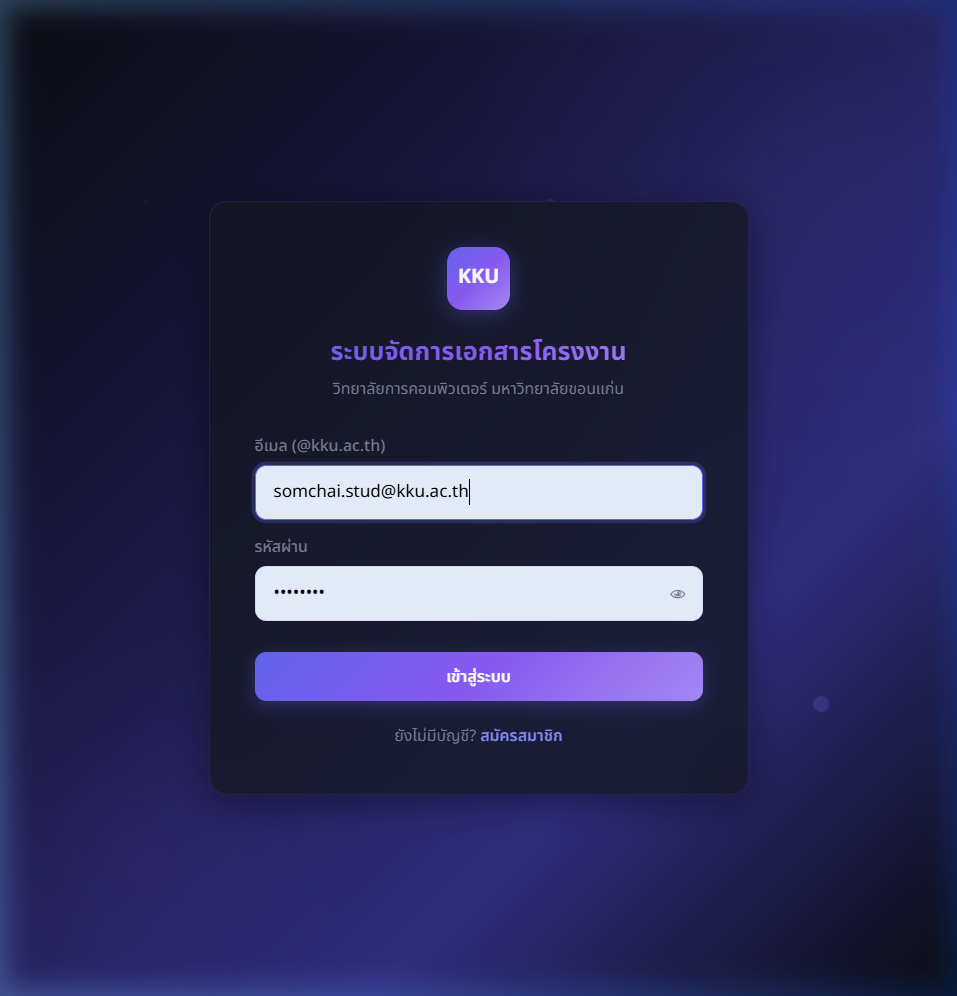
\includegraphics[width=0.5\linewidth]{images/ui-login.png}
\caption{หน้าเข้าสู่ระบบ}
\label{fig:ui-login}
\end{figure}

\section{หน้าหลัก}

หน้าหลักหลังเข้าสู่ระบบแสดงดังภาพที่~\ref{fig:ui-dashboard}

\begin{figure}[H]
\centering
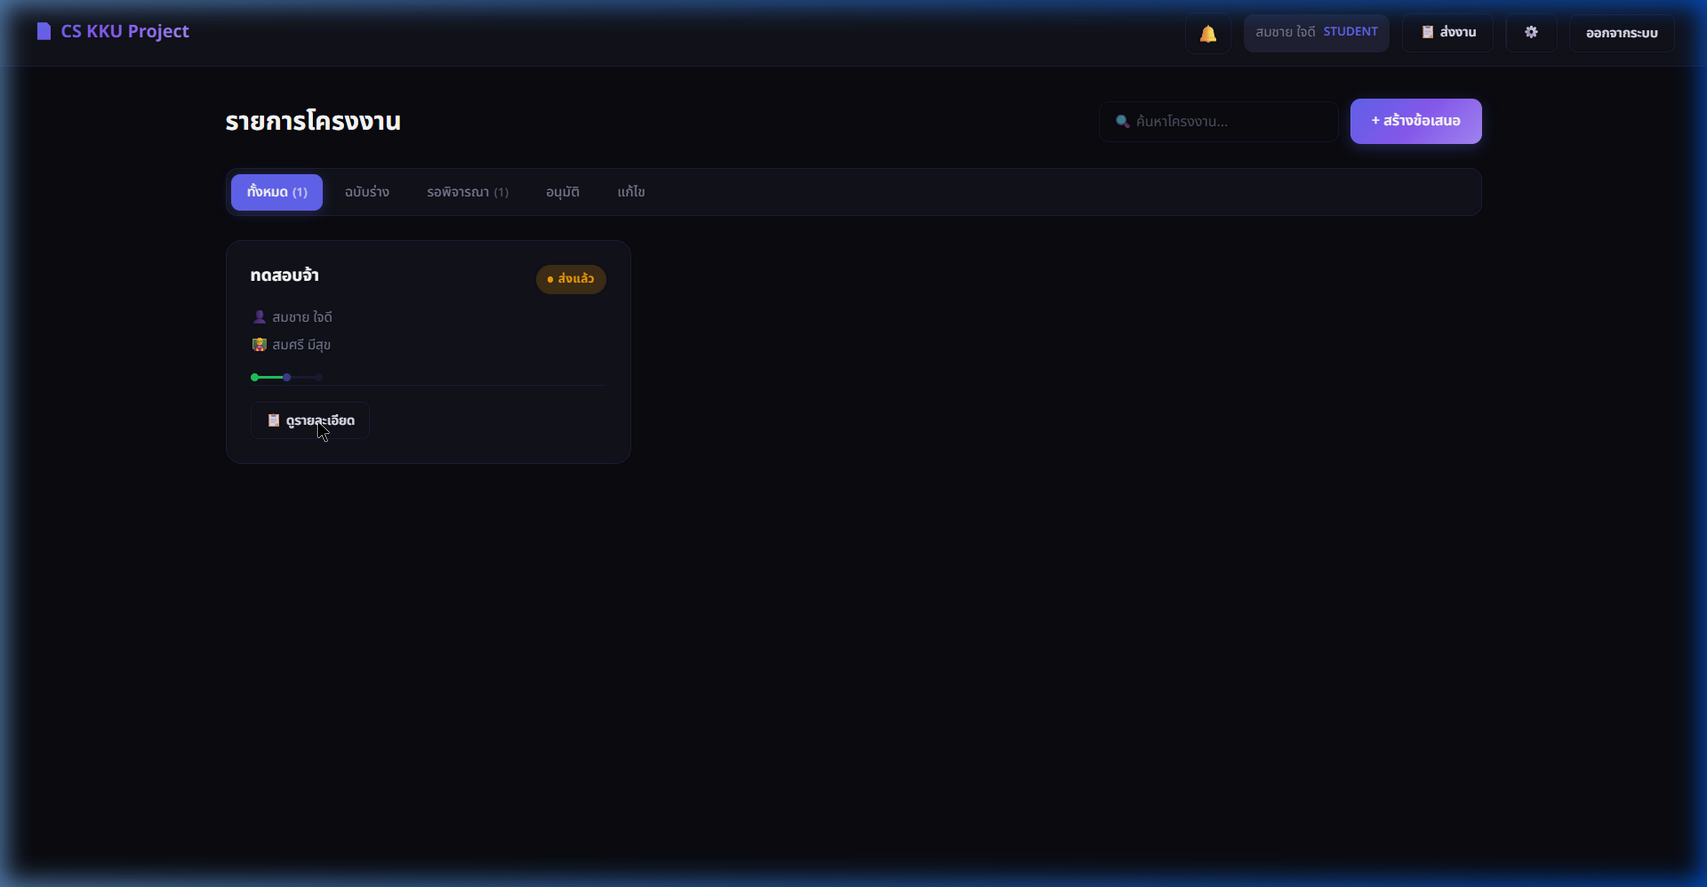
\includegraphics[width=0.95\linewidth]{images/ui-dashboard.png}
\caption{หน้าหลักของระบบ}
\label{fig:ui-dashboard}
\end{figure}


\chapter{คู่มือการติดตั้งระบบ}
% =====================================================================
% ภาคผนวก ข — คู่มือการติดตั้งระบบ (ตัวอย่าง)
% คู่มือการใช้งานฉบับเต็มให้จัดทำเป็นเล่มแยกด้วย template "Template_Manual_2026"
% =====================================================================
\section{ซอฟต์แวร์ที่ต้องติดตั้ง}

\begin{enumerate}
  \item Node.js รุ่น 20 ขึ้นไป
  \item PostgreSQL รุ่น 15 ขึ้นไป
\end{enumerate}

\section{ขั้นตอนการติดตั้ง}

ดาวน์โหลดซอร์สโค้ด ติดตั้งแพ็กเกจ และเริ่มระบบด้วยคำสั่งต่อไปนี้

\begin{lstlisting}[language=bash, deletekeywords={env}, numbers=none]
git clone https://github.com/<user>/<repository>.git
cd <repository>
npm install
cp .env.example .env    # แก้ค่าการเชื่อมต่อฐานข้อมูลในไฟล์ .env
npm run dev
\end{lstlisting}

เมื่อระบบเริ่มทำงานแล้ว เปิดเว็บเบราว์เซอร์ไปที่ \url{http://localhost:3000}


\begin{biography}
% =====================================================================
% ประวัติผู้เขียน (คู่มือข้อ 20) — ไม่เกิน 1 หน้า เป็นหน้าสุดท้ายของเล่ม
% ระบุชื่อ-นามสกุล วัน เดือน ปีเกิด สถานที่เกิด ประวัติการศึกษา
% รางวัลหรือทุนการศึกษา และประสบการณ์ทางวิชาการ (ถ้ามี)
% =====================================================================
\noindent\textbf{ชื่อ-นามสกุล}\quad นาย\ldots{} \ldots{}

\noindent\textbf{วัน เดือน ปีเกิด}\quad \ldots{} \ldots{} พ.ศ. \ldots{}

\noindent\textbf{สถานที่เกิด}\quad จังหวัด\ldots{}

\noindent\textbf{ประวัติการศึกษา}
\begin{enumerate}
  \item พ.ศ. \ldots{} มัธยมศึกษาตอนปลาย โรงเรียน\ldots{}
  \item พ.ศ. \ldots{}--ปัจจุบัน วิทยาศาสตรบัณฑิต สาขาวิชาวิทยาการคอมพิวเตอร์
        วิทยาลัยการคอมพิวเตอร์ มหาวิทยาลัยขอนแก่น
\end{enumerate}

\noindent\textbf{รางวัลและทุนการศึกษา}\quad \ldots{} (ลบหัวข้อนี้ถ้าไม่มี)

\vspace{\baselineskip}
% นักศึกษาคนที่ 2: คัดลอกบล็อกด้านบนมาวางต่อที่นี่ (ลบถ้าทำคนเดียว)

\end{biography}

\end{document}
